%
% File acl2020.tex
%
%% Based on the style files for ACL 2020, which were
%% Based on the style files for ACL 2018, NAACL 2018/19, which were
%% Based on the style files for ACL-2015, with some improvements
%%  taken from the NAACL-2016 style
%% Based on the style files for ACL-2014, which were, in turn,
%% based on ACL-2013, ACL-2012, ACL-2011, ACL-2010, ACL-IJCNLP-2009,
%% EACL-2009, IJCNLP-2008...
%% Based on the style files for EACL 2006 by 
%%e.agirre@ehu.es or Sergi.Balari@uab.es
%% and that of ACL 08 by Joakim Nivre and Noah Smith

\documentclass[11pt,a4paper]{article}
\usepackage[hyperref]{acl2020}
\usepackage{times}
\usepackage{latexsym}
\usepackage{array}
\usepackage{graphicx}
\usepackage{natbib}
\usepackage{float}
\restylefloat{table}
\graphicspath{ {./figures} }
\DeclareGraphicsExtensions{.pdf,.png,.jpg}
\renewcommand{\UrlFont}{\ttfamily\small}

% for coloring
\usepackage{color}
\newcommand{\red}[1]{\textcolor{red}{#1}}
\newcommand{\blue}[1]{\textcolor{blue}{#1}}
\newcommand{\green}[1]{\textcolor{green}{#1}}

% for algorithms
\usepackage[english]{babel}
\usepackage[utf8]{inputenc}
\usepackage{algorithm}
\usepackage[noend]{algpseudocode}
\usepackage{color}
\algnewcommand{\IIf}[1]{\State\algorithmicif\ #1\ \algorithmicthen}
\algnewcommand{\EndIIf}{\unskip}

\usepackage{tabularx}

% This is not strictly necessary, and may be commented out,
% but it will improve the layout of the manuscript,
% and will typically save some space.
\usepackage{microtype}

\aclfinalcopy % Uncomment this line for the final submission
%\def\aclpaperid{***} %  Enter the acl Paper ID here

%\setlength\titlebox{5cm}
% You can expand the titlebox if you need extra space
% to show all the authors. Please do not make the titlebox
% smaller than 5cm (the original size); we will check this
% in the camera-ready version and ask you to change it back.

\newcommand\BibTeX{B\textsc{ib}\TeX}

\title{Typo BERT-ATTACK}

\author{Seungil Lee \\
  KAIST School of Computing\\
  \texttt{silly5921@kaist.ac.kr} \\\And
  Jongchan Park \\
  KAIST School of Computing\\
  \texttt{jongchan.park@kaist.ac.kr} \\\AND
  Eugene Seo \\
  KAIST School of Computing\\
  \texttt{eugene.s21@kaist.ac.kr} \\\And
  Dohyung Kim \\
  KAIST School of Computing\\
  \texttt{sidsince0428@kaist.ac.kr} \\\
  }

\date{\today}

\begin{document}
\maketitle
\begin{abstract}
We suggest \textbf{Typo BERT-ATTACK}, an efficient and effective model generating adversarial examples using both typo and BERT. We addressed the original paper, BERT-ATTACK’s problem, and added typo generation to provide various attack methods. As a result, \textbf{Typo BERT-ATTACK} generates human unrecognizable attack examples, while keeping the strengths of BERT-ATTACK. Through our experiments, the power of using two attack methods is verified. In addition, the optimal ratio between perturbation generated by typo and BERT are found in each dataset. 
\end{abstract}

%-----------------------------------------------------------------------------------
\section{Introduction}

Recently, deep learning has achieved state-of-the-art advances in various topics. Nonetheless, recent adversarial attack works have verified the vulnerability of neural networks. Adversarial attack studies attempt to attack the model to make a mistake via adversarial examples. However, it is not easy to generate fluent adversarial examples on NLP models since the texts are discrete. 

Previous approaches achieved successful attacks by adopting heuristic rules. HotFlip \citep{HotFlip} introduced character-level error in a white-box setup, yet it can attack in a limited boundary. TextFooler \citep{TextFooler} suggested changing the most vulnerable word into its synonym. It used sentence similarity to rank the semantic similarity, but it is still a context unaware.

BERT-ATTACK \citep{BERT-ATTACK:20} solved the previous papers’ limitations via BERT \citep{BERT}. Through BERT, BERT-ATTACK succeeded in generating fluent and semantic-consistent substitutions. Also, it reduced time costs by eliminating perturbation scoring steps. 

\begin{figure}[htbp]
\centering
    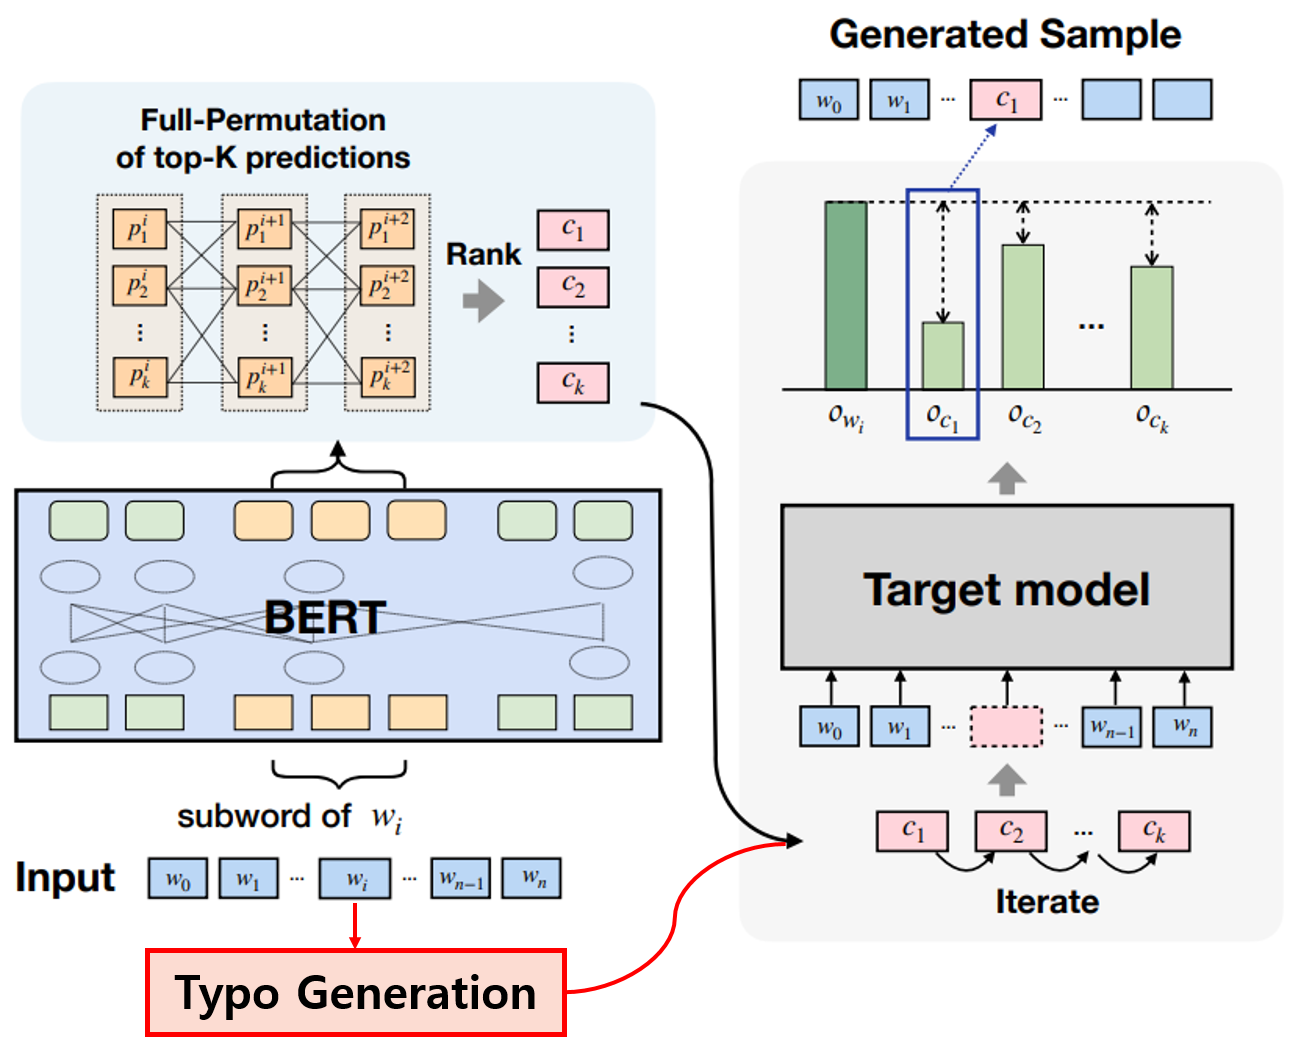
\includegraphics[width=218.268pt]{figure1.png}
    \caption{One step of the replacement strategy} 
    \label{fig:Typo_BERT-ATTACK}
\end{figure}

We propose \textbf{Typo BERT-ATTACK}\footnote{Codes are available here.\\https://github.com/ChoiIseungil/BERT-Attack}, which generates perturbed sentences using typos and BERT. Typos do not preserve the semantic of the original input, but it is difficult for humans to distinguish because it still looks almost identical to the original sentences. To generate appropriate typos, we referred to five methods suggested by \citet{Hagen:17}. In addition, we found various severe problems during replication experiments and modified the code to generate more natural attack examples while keeping the original strengths. 

Experimental results show that \textbf{Typo BERT-ATTACK} has a higher attack success rate than only using BERT-ATTACK. The optimal ratio between perturbations produced using typo and BERT is observed. 
% To summarize our project, we improved the original paper, BERT-ATTACK, and implemented our key idea, Typo BERT-ATTACK. 

%-----------------------------------------------------------------------------------
\section{Dataset}

On our development and experiments, we selected four datasets with a different tasks to test the overall performances of attack model. 
% The fine-tuned models used for the attack are all available on HuggingFace. 
% need to make a table!
\begin{table*}[]
\centering
\begin{tabular}{ll}
\hline \textbf{Dataset} & \textbf{Model} \\ \hline
IMDB                  & fabriceyhc/bert-base-uncased-imdb \\
AG's News             & fabriceyhc/bert-base-uncased-ag\_news  \\
SNLI (p/h)            & boychaboy/SNLI\_bert-large-uncased  \\
HateXplain (3 labels) & Hate-speech-CNERG/bert-base-uncased-hatexplain \\
HateXplain (2 labels) & Hate-speech-CNERG/bert-base-uncased-hatexplain-rationale-two \\
\hline
\end{tabular}
\caption{\label{Model-table} Models used in the experiments. }
\end{table*}

\paragraph{Text Classification}

\begin{itemize}
    \item \textbf{IMDB}\footnote{https://datasets.imdbws.com/} Document-level binary sentiment classification dataset of movie reviews. 
    \item \textbf{AG’s News} Sentence-level news topic classification task by \citet{AG_news}, which can classify world, sports, business, and science. 
    \item \textbf{HateXplain} \citep{HateXplain} Hate speech detection dataset composed of posts on Twitter and Gab. Each post is annotated from three different perspectives: hate, offensive or normal. 
\end{itemize}

\paragraph{Natural Language Inference}

\begin{itemize}
    \item \textbf{SNLI} \citep{SNLI} Stanford natural language inference task dataset. The pair of one premise and one hypothesis sentences are given, and the goal is to predict the hypothesis is whether entailment, neutral, or contradiction.
\end{itemize}

%-----------------------------------------------------------------------------------
\section{BERT-ATTACK Improvement}
\label{sec:BERT-ATTACK Improvement}

Before implementing \textbf{Typo BERT-ATTACK}, we addressed the existing problems in BERT-ATTACK. 

\subsection{Approach}
\label{Improvement:Approach}

BERT-ATTACK attacks a word composed of sub-words as the following. 

\begin{enumerate}
\item Pick top-K predictions for each sub-words
\item Make $K^N$ permutations 
\item Rank them with the perplexity 
\item Use the top-K candidates
\end{enumerate}
 
\noindent However, the official code calculates perplexity for only 24 candidates. We solved this problem by fixing the code, yet the attack time had soared. The reason was the existence of particular words composed of extremely many sub-words.

In addition to the time cost, the original code generated a poor typo on words composed of sub-words. The perturbations on each sub-words resulted in a worse candidate word than a simple typo. Therefore, we limited the number of sub-words that can change. It prevented unacceptable attacks and solved the time-consuming problem.

Third, we filtered out the words containing punctuation marks from the target and the candidate list. The original BERT-ATTACK generated abnormal attack cases that generate a random text from a punctuation mark and vice versa. Those are not valid attacks since humans cannot infer the original test. Through our approach, the attack became natural. 

Lastly, we changed the method of perplexity calculation. The original code calculated the perplexity by putting a single word into BERT. We concluded this is the usage out of the domain since BERT was not trained with single-word sentences. Therefore, we created a phrase containing words of the existing sequence before and after the candidate word, then the phrases are used as the input of BERT. In this way, we maximized BERT’s functionality.

\subsection{Experiment}

We modified original model into 5 different types.
Table \ref{tab:modification_setting} describes our setting for each models.
For baseline models, we only changes the parameter of the original model.
All candidate models are to resolve subword perturbation problem. They don't limit any candidates from subword perturbation, but each model varies the number of generated candidates.
For punctuation problems, we introduce Punc models. They exclude any punctuation related words.
To solve the execution time problem, Subword models limit the maximum subword that can be perturbed during subword perturbation.
Finally, to improve the prediction from BERT, we changed the policy of scoring perplexity. Instead of using the word as input, phrase models use phrase.


With modified models, we experiment its performance with AG's news dataset. 

% Please add the following required packages to your document preamble:
% \usepackage{graphicx}
{\renewcommand{\arraystretch}{1.2}
\begin{table*}[H]
\resizebox{\textwidth}{!}{%
\begin{tabular}{l|ccll|c|c|c|c}
\hline
\textbf{Model name} & \multicolumn{4}{c|}{\textbf{Baseline}}  & \textbf{All candidates} & \textbf{Punc} & \textbf{Phrase} & \textbf{Subword}        \\ \hline
\textbf{Details}    & \multicolumn{4}{c|}{Original Code}                                               & Consider all candidates & Punctuation excluded & Perplexity improvement & Limit subwords \\ \hline
\textbf{Parameter}  & \multicolumn{1}{c|}{\# of candidates} & \multicolumn{3}{c|}{Subword perturbation} & \# of candidates         & Subword perturbation & Length of phrase       & \# of subword
 \\ \hline
\end{tabular}%
}
\caption{Types of modified models}
\label{tab:modification_setting}
\end{table*}
}
\subsection{Result}
\label{sec:improvement}
% Results here
% {\renewcommand{\arraystretch}{1.1}
\begin{table}[hbt!]
\begin{tabularx}{\columnwidth}{X|l|l}
% \begin{tabular}{lll}
\hline
\textbf{Model}   & \textbf{Accuracy} & \textbf{Time}     \\ \hline
Baseline-1       & 0.20     & 1290.8928 \\ \hline
Baseline-2       & 0.20     & 630.5436  \\ \hline
Baseline-3       & 0.23     & 732.7911  \\ \hline
All candidates-1 & 0.20     & 7205.7287 \\ \hline
All candidates-2 & 0.20     & 648.0994  \\ \hline
Punc-1           & 0.30     & 743.0371  \\ \hline
Punc-2           & 0.26     & 705.5875  \\ \hline
Phrase-1         & 0.24     & 644.0462  \\ \hline
Phrase-2         & 0.25     & 655.0946  \\ \hline
Subword-1        & 0.26     & 698.7883  \\ \hline
Subword-2        & 0.23     & 661.3538  \\ \hline
Final-1          & 0.25     & 697.9477  \\ \hline
Final-2          & 0.24     & 664.2827  \\ \hline
\end{tabularx}
% \end{tabular}
\caption{Performance of each modified models}
\label{tab:result_modification}
\end{table}
% }

Table \ref{tab:result_modification} shows our final experiment results.

\begin{itemize}
\item \textit{Baseline}:
We change parameter of original model to generate Baseline models.
Baseline-1 model is equivalent to original model, Baseline-2 model reduces the number of candidates during subword perturbation, and Baseline-3 model doesn't attack with subword.
Among Baseline models, Baseline-1 and Baseline-2 show the best performance. 
Despite of their performance, we decide not to use those models because they are just changed their parameter so that still contains mentioned problems.

\item \textit{All candidates}:
All candidates models don't limit the number of already generated candidates.
All candidates-1 makes 4 candidate per subword, but All candidates-2 makes 2 candidate per subword.
For All candidates models, two models doesn't show the performance gap. 
However, All candidates-1 spends too much execution time.
To solve this problem, we introduce Subword models later.

\item \textit{Punc}:
Because punctuation cannot be positioned anywhere, we don't handle any punctuation.
Punctuation can be related with subword, so we decided to make two model that Punc-1 doesn't perform subword perturbation, and Punc-2 does.
Between two model, Punc-2 shows better performance than Punc-1.

\item \textit{Subword}:
To resolve the execution time problem of All candidates-1, we introduce subword model that limit too many subwords.
Subword-1 uses only two subword during subword perturbation, and Subword-2 uses 3 of them.
By Subword model, we can successfully reduce execution time, and Subword-2 can attack successfully than Subword-1.

\item \textit{Phrase}:
Phrase models improves the performance when model gets perplexity to generate candidates by using phrase rather than word itself.
Phrase-1 and Phrase-2 uses 2 and 3 length phrase each. Both improves the performance, and Phrase-2 model improves much more than Phrase-1 model.

\end{itemize}

Considering the performance of each model, we decided to make 2 different final models. 
Both final models use All candidates-1, Punc-2, and Subword-2.
However, Final-1 model uses Phrase-1 but Final-2 model uses Phrase-2.
Because Final-2 shows the better performance, we use Final-2 for all other experiments.

\begin{table*}[hbt!]
    \centering
    \begin{tabular}{l|c|c|c}
    \hline
    \textbf{Dataset} &
        \textbf{\begin{tabular}[c]{@{}c@{}}Original Accuracy\end{tabular}} &
        \textbf{\begin{tabular}[c]{@{}c@{}}Attacked Accuracy\\ (original model)\end{tabular}} &
        \textbf{\begin{tabular}[c]{@{}c@{}}Attacked Accuracy\\ (new model)\end{tabular}} \\ \hline                                                                      
    AG's News                                                                    & 92.6                                   & 18.4                                              & 26.0                                         \\
    IMDB                                                                         & 93.2                                   & 4.5                                               & 6.4                                          \\
    \begin{tabular}[c]{@{}l@{}}SNLI\\(hypothesis)\end{tabular}                  & 89.5                                   & 33.2                                              & 32.8                                         \\
    \begin{tabular}[c]{@{}l@{}}SNLI\\(premise)\end{tabular}                     & 89.5                                   & 32.8                                              & 33.1                                         \\
    \begin{tabular}[c]{@{}l@{}}HateXplain\\(Toxic/Non-toxic)\end{tabular}       & 79.5                                   & -                                                 & 16.2                                         \\
    \begin{tabular}[c]{@{}l@{}}HateXplain\\(Hate/Normal/Offensive)\end{tabular} & 66.8                                   & -                                                 & 14.9                                         \\ \hline
    \end{tabular}
    \caption{Performances of the all datasets}
    \label{tab:result_alldataset}
    \end{table*}

Table \ref{tab:result_alldataset} shows the performance of all other datasets. 
Since we filter all punctuation, its performance should inevitably become worse. 
However, the number of unnatural attacks are significantly decreased.


\begin{table*}[hbt!]
\resizebox{\textwidth}{!}{%
\begin{tabular}{l|l}
\hline
\textbf{Input sentence}      & \red{teacher} asks \red{class} where is pakistan little johnny \textcolor{red}{replies} outside with paki steve \\ \hline
\textbf{Original model}      & \green{(} asks \green{,} where is pakistan little johnny \green{(} outside with paki steve                                     \\ \hline
\textbf{New model (Final-2)} & \blue{teachers} ask \blue{classes} where is karachi kid jimmy \blue{reacts} outside with katu steve \\ \hline      
\end{tabular}%
}
\caption{Examples of the adversarial attack of the original and new model}
\label{tab:example-final}
\end{table*}
 
\subsection{Example}
In Table \ref{tab:example-final}, there is an example of how models attack the sentence. 
In this example, all changes of original model is related to bracket or punctuation.
However, our new model (i.e. Final-2) doesn't show any punctuation marks during attack.
Therefore, it gives more natural outputs, which are more suitable for adversarial attack.



%-----------------------------------------------------------------------------------
\section{Typo BERT-ATTACK}
\label{sec:Typo BERT-ATTACK}

In this section, we designed the \textbf{Typo BERT-ATTACK} and evaluated its performance.

\subsection{Approach}

We set the result of Section 2 to our new baseline and added the typo attack method to increase the potential of the attack.
We generated attack candidates with five different methods, and the details are the following.

\begin{itemize}
    \item Random Character Insertion     \\ (e.g. ``search typo'' $\rightarrow$ ``search tyapo'')
    \item Random Character Deletion      \\ (e.g. ``search typo'' $\rightarrow$ ``search tpo'')
    \item Random Character Substitution  \\ (e.g. ``search typo'' $\rightarrow$ ``search type'')
    \item Swap Neighbor Character        \\ (e.g. ``search typo'' $\rightarrow$ ``search tyop'')
    \item Swap Adjacent Keyboard Character \\ (e.g. ``search typo'' $\rightarrow$ ``search typi'')
\end{itemize}

\begin{algorithm}[hbt!]
    \centering
    \caption{Typo Generation}
    \label{alg:Typo}
    \begin{algorithmic}[1]
    
    \Procedure{Typo Generation}{word, K}
    % \State $S = [w_0, w_1, ...]$ \textnormal{// input: tokenized sentence}
    \If{length(word) $< 5$}
        \State \Return []
    \EndIf
    \State $C\gets [ ]$ 
    \While{length(C) $< K$} 
        \State {$F \gets$ \textnormal{Randomly chosen typo generation method}}
        \State {$w \gets F$ \textnormal{(word)}}
        \If{w $\not\in$ NLTK scope}
            \State {$C = C + w$}
        \EndIf
    \EndWhile
    \State \Return C
    \EndProcedure
    
    \end{algorithmic}
    
\end{algorithm}

With these typo generations, there might have some ambiguity like `good' $\rightarrow$ `gold'.
It is because applying the above methods can generate the semantically different \textit{complete} words, rather than \textit{typo-like} words. Therefore, we filtered out these candidates with the NLTK WordNet dataset \cite{Princeton_2010}.
NLTK WordNet is the vocabulary-focused English dictionary dataset from Princeton University.
It contains about 160k words and 120k synonym sets.

Also, we used \textit{textattack} library \cite{morris2020textattack} to implement the above typo generation methods.

\textbf{Algorithm 1} describes the Typo Generation strategy.


% \setlength{\intextsep}{1\baselineskip}

\textbf{Algorithm 2} is the pseudocode of the entire process of the \textbf{Typo BERT-ATTACK}.
In the original algorithm, the process works in the following order,
\begin{enumerate}
    \item Searching vulnerable words
    \item Word replacement with BERT
    \item Attacking the given model
\end{enumerate}

Therefore, we add the previous typo generation algorithm, \textbf{Algorithm 1} before Step 3.
% \setlength{\intextsep}{1\baselineskip}
% \setlength{\topfigrule}{0pt}
% \setlength{\textfloatsep}{0pt}

\subsection{Experiment}

Before conducting the experiments on \textbf{Typo BERT-ATTACK}, we designed our custom parameter, $\alpha$. 
It is the proportion of the typo candidates among total candidates.
Equation \ref{eq:alpha} is the expression of the parameter $\alpha$.

\begin{equation}
\label{eq:alpha}
    \alpha = \frac{|\textit{typo candidate}|}{|\textit{typo candidate}| + |\textit{BERT candidate}|}
\end{equation}

We set up the attack experiment using the five different alpha values for each fine-tuned model. We purposed to find the ideal ratio of the typo candidates through this experiment. 


\begin{algorithm}
\begin{center}
\caption{Typo BERT-ATTACK}
\label{alg:TypoBERTattack}
\begin{algorithmic}[1]
\Procedure{importance Ranking}{S} 
\State $S = [w_0, w_1, ...]$ %\textnormal{// input: tokenized sentence}
\State \textnormal{sort S using} $I_{w_i}$ \textnormal{in descending order}
\State \quad \textbf{where} $I_{w_i} = o_y(S) - o_y(S_{\setminus w_i})$ 
\State \quad \,\,$o_y(S) = $ \textnormal{logit output for correct label y} 
\State \Return $S$
\EndProcedure

\Procedure{Replacement}{}
\State $S = [w_0, w_1, ...]$ 
\State $H = [h_0, ..., h_n]$ 
\State $L \gets$ \texttt{Importance Ranking}$(S)$ 
\State $P^{\in n \times K_{bert}} \gets top-K_{bert}$ \textnormal{candidates for all sub\-words using BERT}
\State $S^{adv}=S$
\For{$w_j \in L$}
        \If{punctuation mark $\in w_j$} 
            \State \textnormal{Continue} 
        \EndIf
        \If{$w_j$ is a whole word} 
            \State $C_{bert} \gets Filter \, (P^j)$
        \Else
            % \State $C_{bert} \gets Filter$ \textnormal{(candidates using PPL ranking)}
            \State $C_{bert} \gets Filter$ \textnormal{($PPL(P^j)$)}
        \EndIf
        \State $C_{typo} \gets$ \par
        \hskip\algorithmicindent \texttt{Typo Generation} $(w_j, K_{typo})$ 
        \State $C_{total} = C_{bert} + C_{typo}$ 
        \For{$c_k \in C_{total}$} 
            \If{punctuation mark $\in c_k$} 
                \State \textnormal{Continue} 
            \EndIf
            % \State $S' = S^{adv}[0:j] + [c_k] + S^{adv}[j+1: ]$ 
            \State $S' = S^{adv}$ 
            \State $S'[k] = c_k$ 
            \State $Y\gets $ gold-label
            \If{argmax$(o_j(S')) \neq Y$} 
                \State \Return $S^{adv}=S'$ 
            \Else  
                \If{$(o_j(S')) < (o_j(S^{adv}))$}
                    \State $S^{adv}=S'$ 
                \EndIf
            \EndIf
        \EndFor
        
    \EndFor
    \State \Return \textbf{None}

\EndProcedure
\end{algorithmic}
\end{center}
\end{algorithm}

\subsection{Result}

\subsubsection{Attack Examples}
There are three different cases of attack results.
\begin{itemize}
\item Case 1 is the original BERT-ATTACK succeeded, 100\% Typo-ATTACK failed.
\item Case 2 is the original BERT-ATTACK failed, 100\% Typo-ATTACK succeeded.
\item Case 3 is the original BERT-ATTACK, 100\% Typo-ATTACK failed, only Mixed ATTACK succeeded.
\end{itemize}

The detailed examples are in the Appendix ~\ref{sec:appendix}.
Also, we noticed that the results of Mixed ATTACK is more fluent than the results of 100\% Typo-ATTACK.

\subsubsection{Attacked Accuracy}
{\renewcommand{\arraystretch}{1}
\begin{table*}[hbt!]
    \centering
      
    \begin{tabular}{l|>{\centering\arraybackslash}p{1.5cm}p{1.5cm}p{1.5cm}p{1.5cm}p{1.5cm}|c}
      \hline
      & \textbf{0} & \textbf{.25}  & \textbf{.50}  & \textbf{.75} & \textbf{1}    & \textbf{Original} \\ \hline
  IMDB                                                        & 14.4       & \textbf{7.4}  & 7.6           & 10.3         & 18.5          & 93.2              \\
  AG's News                                                   & 61.0       & 33.4          & 31.6          & 28.8         & \textbf{27.0} & 92.6              \\
  \begin{tabular}[c]{@{}l@{}}SNLI\\ (hypothesis)\end{tabular} & 21.9       & 13.7          & \textbf{13.4} & 15.0         & 22.4          & 89.5              \\
  \begin{tabular}[c]{@{}l@{}}SNLI\\ (premise)\end{tabular}    & 23.2       & \textbf{11.7} & 13.2          & 13.2         & 18.1          & 89.5              \\
  \begin{tabular}[c]{@{}l@{}}HateXPlain\\ (Toxic/Non-toxic)\end{tabular}       & 21.4 & 15.9 & \textbf{13.6} & 14.9 & 24.1 & 79.5 \\
  \begin{tabular}[c]{@{}l@{}}HateXPlain\\ (Hate/Normal/Offensive)\end{tabular} & 21.4 & 9.9  & \textbf{9.2}  & 9.3  & 13.8 & 66.8 \\ \hline
      \end{tabular}
    \caption{Attacked accuracy(\%). The bold typfaces are indicating the best attack}
    \label{tab:results}
    \end{table*}
    }
  
  \begin{figure}
    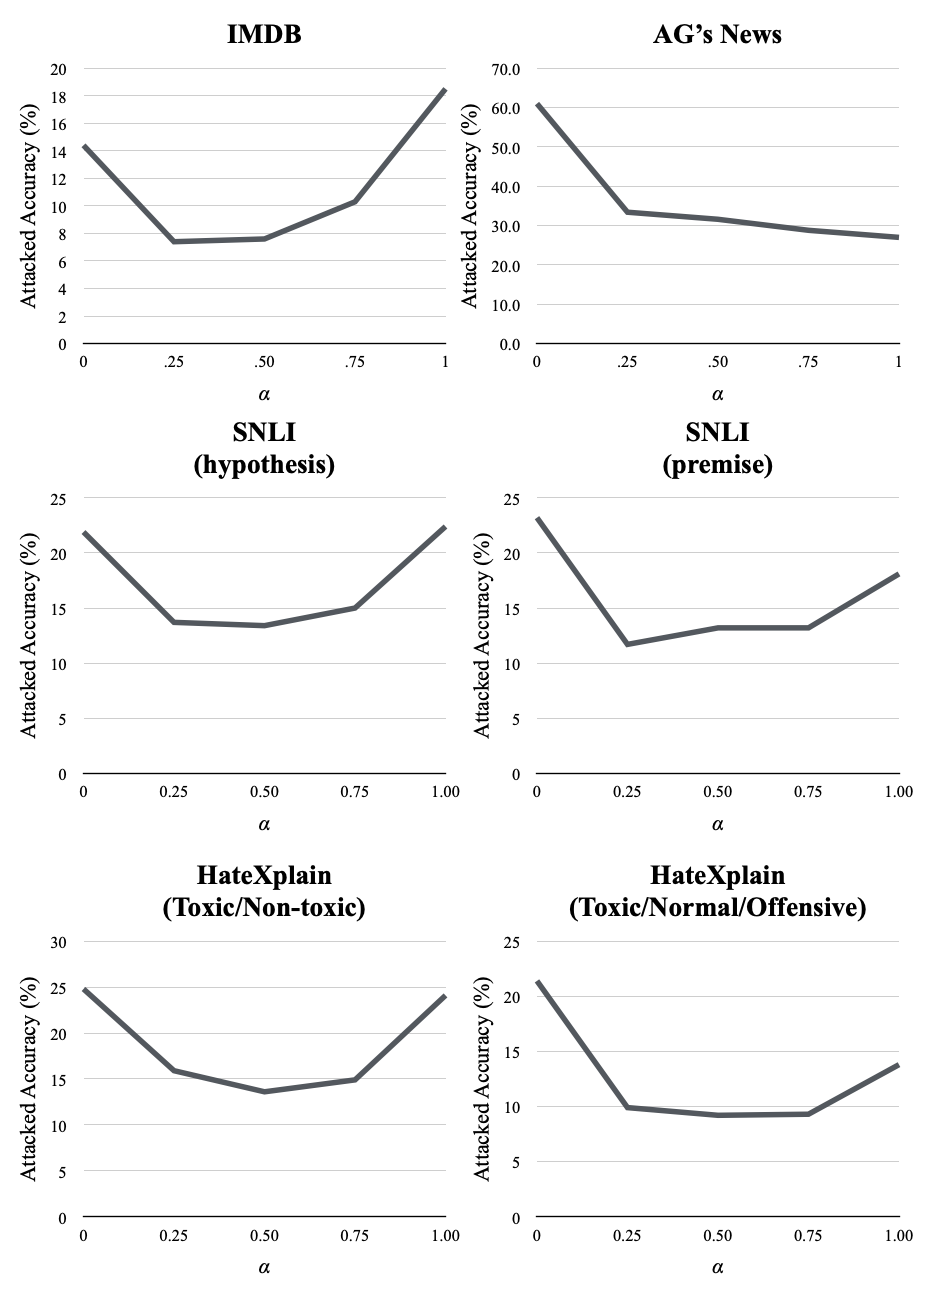
\includegraphics[width=0.5\textwidth]{figure2}
    \caption{Attacked accuracy(\%) of 6 datasets with resppect to $\alpha$}
    \label{fig:results}
  \end{figure}
  
  Table~\ref{tab:results} quantitatively shows attacked accuracies of 30 experiments. The last column is the original accuracies of the new baseline discussed in the Section~\ref{sec:improvement}.
  Remaining five datasets except for AG's News, the optimal $\alpha$ value was lied between 0 and 1.
  100\% typos was the best for the AG's News unlike other datasets.

\subsection{Limitation and Future Work}
Although we tried to make a thorough analysis while implementing \textbf{Typo BERT-ATTACK}, there were two major limitations involved.
\begin{table}[hbt!]
    \resizebox{0.5\textwidth}{!}{%
    \begin{tabular}{l|l}
    \hline
    \textbf{Input sentence}      & A man in a \red{black} tank top \blue{wearing} a red \red{plaid} hat. \\ \hline
    \textbf{Attacked sentence}   & A man in a \red{bmack} tank top \blue{wearnig} a red \red{plyid} hat. \\ \hline  
    \end{tabular}%
    }
    \caption{Examples of the unnatural typos}
    \label{tab:example-unnatural}
    \end{table}

\begin{itemize}
    \item \textbf{Typo unnaturalness} The main reason we adopt typos to make an attack is that, we supposed the typos are difficult to visually detected by human, while it still decieves the neural models. Therefore the most important premise of typos is that it is visually inconspicuous to human. However, contrary to our goal, most of the generated typos were very unnatrual. Let's make an example in Figure~\ref{tab:example-unnatural}. While the word \textit{wearing} is changed to the word \textit{wearnig}, which is not easy to be detected, but word \textit{black} and \textit{plaid} are so easy to be caught by human. These examples are the out of our purpose. The future work will try an approach that restricts typo generation so that humans cannot recognize it well through making reliable human research.
    \item \textbf{Explainability} It is remarkable that we performed better than the existing \textbf{Typo BERT-ATTACK}, the big limitation is the explainability. We could not explain the reason why mixing typos and original method is good at attack. Also we could not figure out while optimal $\alpha$ varies among the dataset. We expect this is due to the unique characteristics of each dataset. Further analysis have to be studied to figure out this reasons.
\end{itemize}

\section{Conclusion}
Through a thorough analysis in Section~\ref{sec:BERT-ATTACK Improvement} and Section~\ref{sec:Typo BERT-ATTACK}, we came to the following conclusions.

First, better than no typos at all. Table~\ref{tab:results} shows that typos always enhances the attack performance. We suppose this is because typos are able to break semantics of the target words very easily, so it helps fooling the neural model. 

Second, typos were not always the best. 100\% typos were not the optimal except the AG's News. There were some optimal value for $\alpha$, and this was quite surprising because we first expected typos are much more superior at attacking the model. Therefore figure ~\ref{fig:results} shows a U-shaped graph in which the attack performance decreases as the difference from the optimal $\alpha$ increases. This result means that the effect of the typos are varying with the characteristics of each dataset, and we suppose this is because the typos are not able to change short and important words, because we limited to create typos only for word with length of 5 or more. 


\bibliography{anthology,acl2020}
\bibliographystyle{acl_natbib}

\newpage
\newpage

\appendix

\section{Appendix: Attack Examples}
\label{sec:appendix}
{\renewcommand{\arraystretch}{1.5}
\begin{table*}[hbt!]
{\small
\begin{tabularx}{\textwidth}{l|X|l}
\hline
\textbf{Type} & \textbf{Sentence}  & \textbf{Label}  \\ \hline
\textbf{Ori}  & Profiling Shaukat Aziz : \blue{economic} reformist - / - PM . Shaukat Aziz , taking over as Pakistan \newline \# 39;s 23rd prime minister on Saturday , is a former private banker credited with infusing new \newline life into an almost bankrupt \blue{economy} .   & World News    \\ \hline
\textbf{BERT} & profiling shaukat aziz : \red{monetary} reformist - / - pm . shaukat aziz , taking over as pakistan \# 39;s \newline 23rd prime minister on saturday , is a former private banker credited with infusing new life \newline into an almost bankrupt \red{economics} . & Business News \\ \hline
\textbf{Typo} & prof\red{ll}ing shauka\red{m}t aziz : e\red{q}conomic reformitt - / - pm . shauat aziz , taki\red{b}g over as \red{ap}kistan \# \newline 39;s 23rd p\red{e}ime miniter on \red{as}turday , is a former priva\red{y}e bank\red{re} \red{e}redited with infusin\red{d} new life
\newline into an almost ba\red{d}nkrupt econo\red{n}y .  & World News    \\ \hline
\end{tabularx}
}
\caption{Examples of Case 1. Original BERT-ATTACK succeeded / 100\% Typo ATTACK failed }
\end{table*}
}

{\renewcommand{\arraystretch}{1.5}
\begin{table*}[hbt!]
{\small
\begin{tabularx}{\textwidth}{l|X|l}
\hline
\textbf{Type} & \textbf{Sentence}  & \textbf{Label} \\ \hline
\textbf{Ori}  & Giddy Phelps Touches \blue{Gold} for First Time . \blue{Michael} Phelps won the gold medal in the \blue{400 individual medley} and set a world record in a \blue{time} of \blue{4 minutes} 8.26 \blue{seconds} . & Sports News   \\ \hline
\textbf{BERT} & iddy phelps touch \red{silver} for first times . \red{mike} phelps won the golden award in the \red{butterfly 400 aquatics} and sets a world records in a \red{hours} of \red{7 min} 8.26 \red{min} .      & Sports News   \\ \hline
\textbf{Typo} & \red{k}giddy ph\red{le}ps t\red{b}uches gold for first time . m\red{k}chael phelp won the gold m\red{t}dal in the 400 individ\red{k}al medl\red{ye} and set a world ecord in a time of 4 m\red{k}nutes 8.26 seconds .  & Business News \\ \hline
\end{tabularx}
}
\caption{Examples of Case 2. Original BERT-ATTACK failed / 100\% Typo ATTACK succeeded}
\end{table*}
}

{\renewcommand{\arraystretch}{1.5}
\begin{table*}[hbt!]
{\small
\begin{tabularx}{\textwidth}{l|X|l}
\hline
\textbf{Type} & \textbf{Sentence}$\qquad$(Premises: a woman holding a scruffy cat.) & \textbf{Label} \\ \hline
\textbf{Ori}  & Hypothesis: An \blue{elderly lady} holding a scruffy \blue{dog} and smiling contently .     
& Contradiction \\ \hline
\textbf{BERT}  & Hypothesis: An \red{aged female} holding a scruffy \red{hound} and smiling contently ."    & Contradiction \\ \hline
\textbf{Typo}  & Hypothesis: an elde\red{j}ly lady h\red{lo}ding a \red{cs}ruffy dog and smilin\red{j}g content\red{yl} .    & Contradiction \\ \hline
\textbf{Mixed} & Hypothesis: an e\red{p}lderly \red{female} holdi\red{h}g a scruffy dogs and smili\red{m}g contently . & Entail        \\ \hline
\end{tabularx}
}
\caption{Example of Case 3. Original BERT-ATTACK \& Typo ATTACK failed / Mixed ATTACK succeeded}
\end{table*}
}



\end{document}
